\Chapter{SYNTHETIC DATA GENERATION}\label{sec:Syn}


Simulated data has been playing an increasingly important role in EDM \citep{JEDM:baker2009}. The availability of new simulation software is contributing to this trend in every domain. As an example \citet{jafarpour2015quantifying} used simulated data for disease outbreak detection where simulated data is generated from a hypothesized model of a phenomena. The framework of this study relies on synthetic data. Getting back to the main contribution of this thesis, we proposed an approach for model selection that relies on synthetic data. Using synthetic data allows us to validate the sensitivity of the model selection approach to data specific parameters such as sample size and noise. Then the process of generating data should be accurate such that both data  and model specific parameters are applied properly. Every model studied here can be considered \textit{generative}, to the extent that they can generate synthetic data.

A unique advantage of synthetic data is that the model parameters can be predefined. Once the simulated data is generated with predefined parameters, a model can be trained over the generated data and a comparison with the original, known parameter values becomes possible. This may be the strongest benefit of synthetic data in assessing model fit. Since the hypothesis of this research relies on comparison the performance vector of real vs. synthetic data, then we can also consider data specific parameters of the real data in the generation process to make a better comparison of the results.

\section{Data generation parameters}
%(2) explain how they are either derived from data, or initialized (presumably from a random distribution); 
As described before, there exists two types of parameters for student test outcome:
\begin{itemize}
\item Model specific: These parameters are dependent on the ground truth of a dataset. Skills assessment models that were described in section \ref{SkillsAssessmentModels} considers different parameters. Depending on the type of student model, some of them may share a parameter such as Q-matrix for multiple skills models but still the interpretation of each model is unique. Generally an experiment should be designed to learn these parameters form a dataset or they can be generated under specific criteria. More details for each parameter is given later in this chapter.
\item Data specific (contextual): Regardless of the ground truth of a dataset, there are parameters that describe the dataste's specifications such as number of students. These parameters are common for any student model. They could possibly affect the performance of a model over a dataset. 
\end{itemize}


Table \ref{tbl:param-DataGen} shows a complete list of both types of parameters required for data generation.

\newcommand{\tabitem}{~~\llap{\textbullet}~~}
\newcommand\VRule[1][\arrayrulewidth]{\vrule width #1}



\begin{table}
  \centering

\begin{tabular}{c|c|l!{\VRule[1.5pt]}l|l!{\VRule[1.5pt]}l|}
\multicolumn{3}{c}{}&\multicolumn{3}{c}{Parameters}\tabularnewline
\cline{4-6}
\multicolumn{3}{c!{\VRule[1.5pt]}}{Skills Model}&\multicolumn{2}{c!{\VRule[1.5pt]}}{Model specific}&\multicolumn{1}{c|}{Data specific}\tabularnewline
\cmidrule[1.5pt]{2-6}
&&NMF Conj. & & &  \tabularnewline
\cline{3-3}
&&NMF Add.&&\multirow{-2}{*}{ \tabitem  Q-matrix }&\multirow{-2}{*}{\tabitem Number of students } \tabularnewline
\cline{3-4}
&&DINA& \tabitem Slip & &\tabularnewline
\cline{3-3} 
&\multirow{-4}{*}{\begin{sideways} \scriptsize Multiple\end{sideways}}&DINO& \tabitem Guess&\multirow{-2}{*}{  \parbox[t]{3cm}{ \tabitem Students skills  \\ mastery matrix}}& \multirow{-2}{*}{\tabitem Number of items } \tabularnewline
\cmidrule[1.5pt]{2-5}
&&&\multicolumn{2}{l!{\VRule[1.5pt]}}{\tabitem Student ability  } &  \tabularnewline
&&&\multicolumn{2}{l!{\VRule[1.5pt]}}{\tabitem Item difficulty  } &\multirow{-2}{*}{\tabitem Number of skills } \tabularnewline
&&\multirow{-3}{*}{ IRT}&\multicolumn{2}{l!{\VRule[1.5pt]}}{\tabitem Item discrimination}  &\tabularnewline
\cline{3-5}
&&&\multicolumn{2}{l!{\VRule[1.5pt]}}{\tabitem Student Odds  } & \multirow{-2}{*}{\tabitem Test success rate }  \tabularnewline
&\multirow{-5}{*}{\begin{sideways} \scriptsize Single \end{sideways}}&\multirow{-2}{*}{ Expected}&\multicolumn{2}{l!{\VRule[1.5pt]}}{\tabitem Item Odds}  &  \tabularnewline
\cmidrule[1.5pt]{2-5}
&&&\multicolumn{2}{l!{\VRule[1.5pt]}}{\tabitem Initial Odds } & \multirow{-2}{*}{\tabitem Student score Variance} \tabularnewline
&&&\multicolumn{2}{l!{\VRule[1.5pt]}}{ \tabitem Odds ratio } & \tabularnewline
\multirow{-9}{*}{\begin{sideways} \scriptsize Contributed skills \end{sideways}}&\multirow{-3}{*}{\begin{sideways} \scriptsize Zero\end{sideways}}&\multirow{-3}{*}{ POKS }&\multicolumn{2}{l!{\VRule[1.5pt]}}{\tabitem PO structure}& \multirow{-2}{*}{\tabitem Item score Variance} \tabularnewline
\cmidrule[1.5pt]{2-6}
\end{tabular}
  \caption{Parameters involved in synthetic data generation}
  \label{tbl:param-DataGen}
\end{table}

\subsection{Assessing parameters}

To generate artificial data a set of parameters is required There are two approaches to assess required parameters to generate synthetic data:
\begin{itemize}
\item Parameters borrowed form a real data: Deriving contextual parameters from a real data is a straight forward task. To get model specific parameters we need to learn them from a real dataset given a model. In some cases there exists a predefined (or expert defined) parameter associated with the real data such as expert defined Q-matrices.
\item Generate parameters randomly based on a distribution: In the case that there exists no reference dataset to derive parameters we can randomly select some samples based on a distribution (for example normal distribution). Some parameters have specific conditions that if they become violated it changes the definition of the parameter. More details is given in next sections.

\end{itemize}


The rest of this chapter describes the data generation process based on each model assessment technique that is used in the proposed model selection approach.
% we can also specify which paramters has been borrowed from real data and which one has been generated

\section{POKS}
POKS is a technique that categorized as a ``zero skills'' method does not directly attempt to model underlying skills but instead rely on observable items only. 

\subsection{Obtaining parameters}
This model has three parameters with which the inference in possible : Knowledge structure, Initial probabilities, Odds ratio. To extract these parameters from an existing data we use POKS \footnote{http://www.professeurs.polymtl.ca/michel.desmarais/Papers/UMAP2011/lib-poks.R} R package to learn all the parameters given a dataset. In the case that the data in not available we will generate the parameters first. Below we will describe how these parameters are generated with different conditions and constraints.
%\note{Suggestion: (1) formally define all the parameters of the simulation,
\subsubsection{Knowledge structure(KS)}
This parameter shows the relation and dependency among a set of items. In fact, it reflects the order of learning a set of items in the same problem domain. Assuming items as different ``nodes'' in the structure there is a kind of ``parent-child'' relation between pairs of nodes where an easier item can be the child of a harder item. In our study this relation and dependency is considered as a ``link'' between pair of items. This link is not necessarily exists between each pair. Only those items that are related in the learning process can have a pairwise link. 
The graphical demonstration of knowledge structure is an directed graph with no cycles allowed, except for symmetric relations. Also in the current version of POKS transitive relations between items are explicitly ignored. % because there is a likely strong correlation from transitive to direct relations that would need to be taken into account.

% if you don't have transitive relation in your process you need to state that please


There are few other parameters involved in the generation of KS which are:
\begin{itemize}
\item Number of independent graphs: Even in a set of items there could be different groups of nodes without any dependency between them. Since there is no link between each group them they create an in dependent graph in the knowledge structure. This parameter can also affect the total number of links in a structure where more independent groups results in less number of links in the structure given same density of links in each group. 
\item Total Number of links: This has a correlation with the previous parameter but still we can control the number of dependencies in a KS. This parameter has an direct effect on test success rate and item score variance. Fewer number of links will result in lower test success rate and item score variance.% There are still some other parameters that could change the test success rate and item score variance.
\end{itemize}

%Other input parameters can make the random generation more specific,such as the number of links and number of independent trees in a KS\note{?? Needs to be defined.}. These parameters will change the item variance in the test result matrix. 

\begin{figure}[t]
\centering 
\subfigure[Adjacency matrix ]{  $\begin{array}{ccc}
&\begin{array}{ccccc}
i_{1} & i_{2} & i_{3} & i_{4}& i_{5}\end{array}&\\
\begin{array}{c}
i_{1}\\
i_{2}\\
i_{3}\\
i_{4}\\
i_{5}
\end{array}&\left[\begin{array}{ccccc}
0 & 0 & 0 & 0 &1\\
0 & 0 & 1 & 0 &0\\
0 & 0 & 0 & 1 &1\\
0 & 0 & 0 & 0 &0\\
0 & 0 & 0 & 0 &0
\end{array}\right]&\\
&&\\
&&
\end{array}$}
\qquad
\qquad
\subfigure[Graphical representation ]{ $\begin{array}{cc}
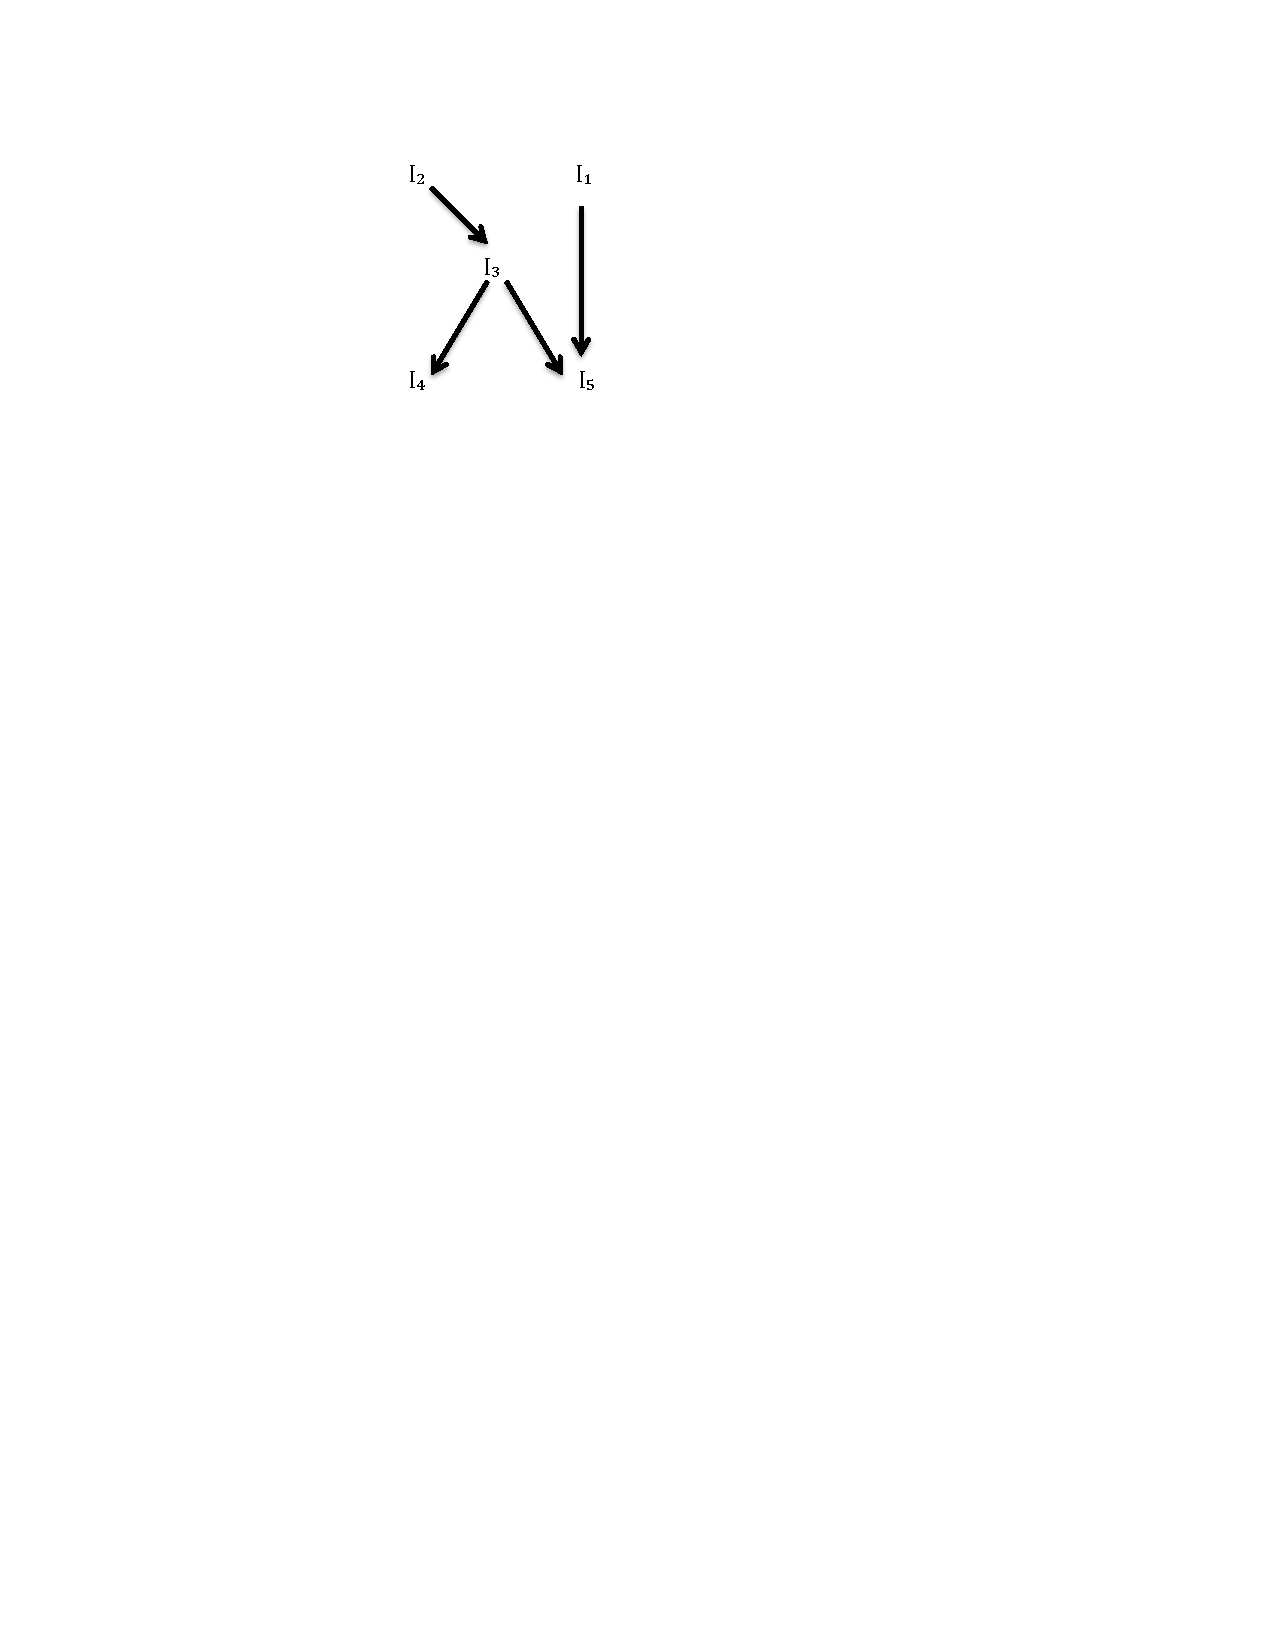
\includegraphics[trim=7cm 20.4cm 11cm 3.5cm,width=.20\linewidth]{SampleKS} &
\end{array}$}

\label{fig:KSExample}
\caption{An example of random KS with 5 items}
\end{figure}

Adjacency matrix  is one way to represent the KS. To avoid having a cycle in the structure we randomly assign $0$-$1$ values to an upper triangular of this matrix. For simplicity we consider the structure to be a single connected graph and the number of links corresponds to half of cells of the upper triangular of this matrix. figure \ref{fig:KSExample} shows a adjacency matrix associated with its graphical structure. 

Once the KS is generated we should assign proper value to each item as an initial value and to each pair of items as odds ratio. One of the important concepts in assigning values to initial probabilities and odds ratio (explanation is in the next subsection) is the ``level'' of a node in the graphical representation of the KS which corresponds to the longest path from that node to a leaf node. A leaf node is a node that does not have any child and a root is a node without any parents. Equation \ref{EQ:Level} shows the definition of this function where $length-of$ returns the length of a path between two nodes and $path$ returns true value if there exists a directed path between two nodes and $leaf$ returns true if the node is a leaf.  For example in figure \ref{fig:KSExample} $I_{5}$ is a leaf with the level of $1$ and $I_{2}$ is a root with level of $3$.

\begin{equation}
L(KS,N_{i}) = max(E|E=length-of(N_{i},p)  ,  \exists path(N_{i},p)  , leaf(p)=True)
\label{EQ:Level}
\end{equation}

%The generation of a random KS consists in randomly assigning 0-1 values to an upper triangular adjacency matrix. \annote{Once the KS adjacency matrix is created, we can assign values to each item that contributes with the initial odds of each node and odds ratio between a pair of nodes.}{not clear; odds ratio has not yet been introduced}

\subsubsection{Initial Probabilities}
%first you have to get probabilities and which probability do you start with? where do they come from?

Each item should be associate with an initial probability of success. This probability has a direct correlation with the difficulty of the item. In general if node $A$ implies node $B$ ($A \rightarrow B$) then node $B$ should have a higher initial probability of success because in this relation item $A$ is the harder problem. The allocation of initial values to items should be done respect to this characteristic. 

Starting from a root node in KS we assign a random initial probability  for each node $N_{i}$ from a range of values between $r_{max}$ to $r_{max}+\frac{1-r_{max}}{L(KS,N_{i})}$ where $r_{max}$ is the maximum initial probability of $N_{i}$ parents. For a node that is a root $r_{max}$ is $0$ since it is starting node and obviously should have the lowest initial probability among its descendant. Also for a leaf the assignment range will be between $r_{max}$ and $1$ because it has level of $1$. 

As mentioned before, the initial probability of success for items come from these values. This set of values changes when a sample is assigned to each item. The process of sampling preforms item by item and in each step a new set of values are assigned to items as the probability of success. This set of probabilities is called the ``state'' of probabilities (shown as $S$ where $S_i$ is the probability of success for item $i$). In this context we use odds instead of probabilities where $O(H) = \frac{P(H)}{1-P(H)}$. The details for changing the ``state of odds'' and assigning samples to items is given in next sections.

\subsubsection{Odds ratio}

The very last parameter is the odds ratio which is a ratio that represents the strength of a link between a pair of items. In the inference for POKS model this parameter is used to update the initial probability of inferred items given a set of observations. The same situation as inference we use this parameter to update the state of odds once an item has been sampled (more on these implementation details is given in the next section).
For inference in POKS, the probability update for node $H$ given $E_1$,... $E_n$ can be written in following posterior odds form:
%\note{This is not a clear description of the process.  What are the $E_i$ here? How is the first $E$ chosen and what is its initial probability? etc...}
\begin{equation}
O(H|E_1,E_2, ... , E_n) = O(H) \prod_{i}^{n} \frac{P(E_i|H)}{P(E_i | \overline{H})}
\label{EQPOKSratio}
\end{equation}
where odds definition is $O(H|E) = \frac{P(H|E)}{1-P(H|E)}$ and $O(H)$ is the initial odds of node $H$. If evidence $E_i$ is negative for observation $i$, then the ratio $\frac{P(\overline{E_i}|H)}{P(\overline{E_i}|\overline{H})}$ is used. we will follow the same steps to generate data based on POKS model. 
There are two types of odds ratio in the POKS model. Assuming $I_{3}$ as a node that has two children and a parent in figure \ref{fig:KSExample}. if the sampling result for this item (with respect to its initial odds) becomes $1$ (or success) then we should update the odds of its children because a success for a harder item should increase the chances of success for an easier one. Therefore we define a ``true odds ratio'' which is applicable when the evidence (in this case the evidence is the one that has been sampled,  node $I_{3}$) becomes a success. If the evidence is $0$ (or failure) then we should update the odds of its parents since a failure for an easier problem should decrease the chances to success a hard one. To update the parents' odds we use ``False odds ratio'' when the evidence is false. In fact $\frac{P(E_i|H)}{P(E_i | \overline{H})}$ in equation \ref{EQPOKSratio} represents the odds ration for item $H$ given evidence $E_i$. 

In our experiments we assigned random values greater than $0.5$ as ``true odds ratio'' and smaller than $0.5$ for ``false odds ratio''for those pairs of items that have link in KS.

%\note{Shouldn't you differenciate between the KS definition and the data generation?  Because KS can be taken from an existing data set, or generated at random with the procedure explained. Then comes the data generation part.}
\subsection{Data generation}

% (3) explain the algorithm for data point generation (should start with nodes that have no parents, then pick nodes for which all parents have values, etc.).  And what about nodes that have many parents?  This is the tricky question since POKS does not define multiple parents conditional probability tables---presumably this means that one parent is picked at random and that creates undeterminism of a kind, since picking one or the other parent would yield different probabilities.  And what about transitive relations?  In practice they are removed in the current POKS software if I recall correctly.  It would need to be explicitely mentioned.  Actually I see that the next paragraph addresses some of these issues.}

Previous sections explained the process of obtaining a pre-defined or a random generated set of parameters for POKS. In this section we explain the process for sampling data points values to create an artificial student test result matrix given a set of parameters. Each record in this approach represent a student test result that requires $n$ iterations to be generated where $n$ is the number of items and the final result matrix needs $m$ (number of students) records. The process simply follows steps in algorithm \ref{POKS:ALG}. Line 8 to 15 of this algorithm updates the state probability of the items. It is important to note that we just look at the neighbors of the item that is sampled. In other words the update propagate in breadth.


\begin{algorithm}
\caption{POKS data generation}
\label{CHalgorithm}
\begin{algorithmic}[1]
\For{each record $i$ \Pisymbol{psy}{206} $m$ (number of students) }
\State or.f = False Odds Ratio
\State or.t = True Odds Ratio
\State  $S$ = Initial odds
\For{each item $j$ \Pisymbol{psy}{206} $n$ (number of items) }
\State Randomly pick item $j$ that has not been sampled
\State $R_{ij}$ =  Sample item $j$ for record $i$ with respect to $S_j$
\If{$R_{ij} = 1$}
\State $U =$ children of item $j$ in $KS$
\State  $\forall c\in U$ :  $S_c = S_c\times or.t_{cj}$
\EndIf
\If{$R_{ij} = 0$}
\State $U =$ parents of item $j$ in $KS$
\State  $\forall p\in U$ :  $S_p = S_p\times or.f_{pj}$
\EndIf
\EndFor
\EndFor
\end{algorithmic}
\label{POKS:ALG}
\end{algorithm}

%The approach for assigning values to each sample is using probabilities for each node and a ratio for each pair for nodes which represent the strength of the link.  Based on the knowledge structure that has been picked \note{picked out of what? it is either inferred from data or generated at random, no?} we can also assess a set of initial probability for each node where a parent node gets a lower initial probability than its children. Inference in the POKS framework to calculate the node's probability relies on standard Bayesian posteriors under the local independence assumption. 

%All the parameters containing Partial Order structure, initial odds and odds ratio can also be obtained form a real dataset. For the case that these values are not predefined we need to assign random values with respect to the defined partial order structure. Once these values are defined, we can pick a node to sample with it's initial odds and consequently update it's neighbors' odds with equation~\ref{EQPOKSratio}. This process could be continued until there exists no node to sample.

% the updates are done based on deepth first or bearth first? how? describe clearly
%\note{This is not clear.  Does it mean that after each new $E_i$ ``observed'', a nodes probability is updated?  For eg. Say we have this: $a \rightarrow b, a \rightarrow c, b \rightarrow d, c \rightarrow d$. if $a=1$ and $b$ gets updated, then $c$, will the probability of $d$ be updated from the posterior based on the observation of $a$ and $b$, or only one of them?  But presumably not based on $a$ as evidence also (if transitivity was removed.  And do you ensure that $d$ will not be assigned (observed) before both $c$ and $b$ are assigned? }

\subsection{Data specific parameters}

Obtaining the performance of different models over a dataset is a main part of our contribution in this study. Some models require number of skills to learn their parameters such as DINA. Since POKS generated dataset does not directly attempt to model underlying skills we have to have a prediction for this important parameter to associate with the data. \citet{Beheshti2012Numbers} proposed two approaches based on factorization technique to predict an optimum number of skills given a dataset. 

The only way to control the test result success rate and student/item score variance is to apply changes on the initial odds of items which are used to sample student test result. For student scores variance, for each record the initial odds can be scaled such that the distribution of the initial odds stays the same; for example we can double all the initial odds to represent a student with higher success rate but still the distribution of items score variance remains the same. Changing the initial odds that follows a specific distribution will create a dataset in which the item variance is following that distribution. It is important to note that this change should not violate any relation in the KS. For overall successrate the initial odds can be scaled independent from students or item perspective, for example tripling all initial odds for all students will result in a higher success rate than the default values.



%The method that generates synthetic dataset based on the POKS model requires a knowledge structure (KS). In this process the KS can be obtained from a real data set which allows us to make a better comparison of the results. It can also be generated as a random KS.  


\section{IRT}

Equation~\ref{IRTEQ} shows the probability of a student given the ability of $\theta$ to success item $j$ which has the difficulty of $b_j$ and discrimination of $a_j$ based on IRT-2PL model. To generate a dataset that follows this model, we need to generate a sample of students with different abilities and items with different difficulties and discriminations. 
\begin{equation}
P(X_j\!=\!1\;|\;\theta) = \frac{1}{1+e^{-a_j(\theta-b_j)}}
\label{IRTEQ}
\end{equation}
\[-4 < \theta < 4\]
\[-3 < b_j < 3\]
\note{what about $a_j$?}

\note{Actually, it would be better to write this with equations, including the Poisson distribution.  See this paper (equation 2 and below): \url{http://educationaldatamining.org/EDM2011/wp-content/uploads/proc/edm2011_paper35_full_Desmarais.pdf}}

Students ability to answer questions and item difficulty are generated by a normal distribution with the mean of $0$ and standard deviation of $1.25$\note{why these numbers?  Shouldn't they be from the sample}. Discrimination (slope or correlation) representing how steeply the rate of success of individuals varies with their ability. In IRT-2PL, the values for discrimination are following a Poisson distribution with lambda parameter set to 10 that kept most values between 0.5 and 3. 

Item discrimination is a parameter that is learnt from training set. A perfect dataset that doesn't have any noise estimates this parameter with extremely large or small values (for example $300$ or $-300$)  which results in an unrealistic outcome prediction. For this purpose we add small amount of noise to prevent this condition.

\section{Linear NMF Conjunctive}

%Further studies with real data will be necessary, granted the results of the existing study warrants such work.

%We will consider that skills have a difficulty level. That difficulty will transfer to items that have this skill. The difficulty of the two-skills items will further increase by the fact that they require the conjunction of their skills. We 

%Examinees need to be assigned ability levels. The ability is, in fact, reflected by the set of skills mastered. , and the assigned ability level will increase this variance over the variance resulting from skill difficulty.

%Finally, two more parameters are used in the simulated the data, namely the $\mathit{slip}$ and $\mathit{guess}$ factors.  They are essentially noise factors and the greater they are, the more difficult is the task of inducing the Q-matrix from data.
%Skill difficulty and examinee ability are each expressed as a random normal variable. The probability density function of their sum provides the probability of mastery of the skill for the corresponding examinee. The skill vector is a sampling in \{0, 1\} based on each skill probability of mastery. 


The very first step to generate simulated test result for linear models is to define a Q-matrix that maps $k$ skills to $n$ items. The Q-matrix can be an expert predefined matrix or a random generated matrix. In the case of unavailable predefined Q-matrix, we defined a Q-matrix that provides all the possible combination of $k$ skills with a maximum of $Max$ skills per item, and at least one skill per item. A total of $\sum\limits_{k=1}^{Max} \dbinom{n}{k}$ items span this space of combinations for example $21$ items for 6 skills and maximum 2 skills per item. This matrix is shown in Figure~\ref{figqmatrixandResutM}. Items 1 to 15 are two-skills and items 16 to 21 are single-skill. Once the Q-matrix is created we can randomly replicate or eliminate some items to adjust the number of items to the desired number. 

\begin{figure}[ht]
\centering

\subfigure[Q-matrix of 6 skills]{
   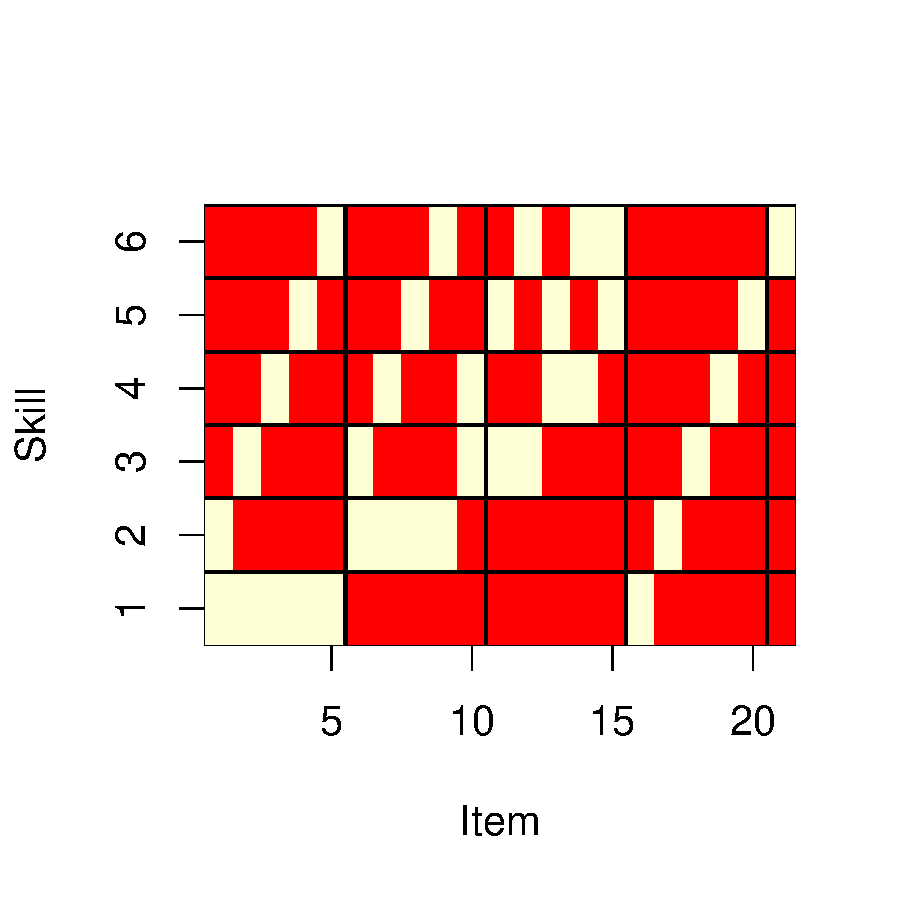
\includegraphics[scale =0.5] {ExpectedQ.pdf}\label{PerfectQ}
 }\quad
 \subfigure[Synthetic data of 100 students with 10\% slip and 20\% guess factor]{
   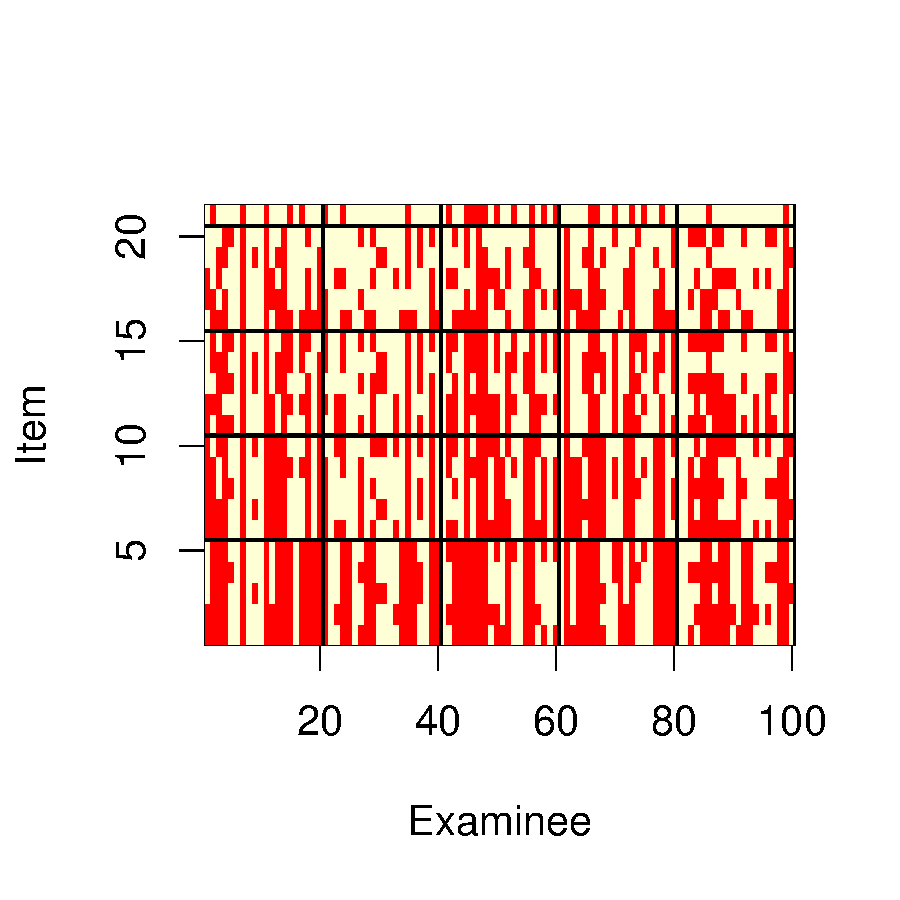
\includegraphics[scale =0.5] {ResultM.pdf}
 }
\caption{Q-matrix and an example of simulated data with this matrix.  pale cells represent 1's and red ones represent 0's.}
\label{figqmatrixandResutM}
\end{figure}

There are two ways to apply item variance in the simulated data and both of them are based on manipulating the values of the Q-matrix. Applying skills difficulty on skills would transfer the difficulty to items that have this skill. The other method is to consider the same weight for skills difficulty but controlling the item variance by assigning different number of skills to items. For example items with 1 skill would become easier to answer comparing to items with two or more skills where skills difficulty is the same for all skills. 

The second step is to create a student skills mastery matrix which maps $k$ skills to $m$ students. In terms of ability for examinees we assigned random values to skills for students but  student variance show up as the variance in number of skills across examinees. At the same time we can apply the overall success rate on the skill mastery matrix using a threshold to discrete the assigned values in skills mastery. 

Once the Q-matrix and Skills mastery matrix is created we can produce the test result matrix with equation~(\ref{eq:6}). The last step is to add slip and guess factors which are set as constant values across items.

A sample of the results matrix is given in figure~\ref{figqmatrixandResutM} where pale cells represent a value of 1 and red cells are 0. Examinee ability shows up as vertical patterns, whereas skills difficulty creates horizontal patterns. As expected, the mean success rate of the 2-skills items 1 to 15 is lower than the single skill items 16 to 21.

\section{Linear NMF Additive}

The process to create synthetic data based on additive type of Q-matrix is almost the same as Conjunctive one. The difference is on the interpretation of the Q-matrix that changes the step where the result matrix is producing.

For this case each cell in the Q-matrix should be normalized on the bases of items. Although each skill has a specific weight to success an item but in our experiment we consider equal weight for all skills of an item. For this purpose all the values assigning to each item in Q-matrix should be divided by the number of involved skills for that item.

\begin{figure}[h]
\begin{tabular}{c}
\subfigure[{Additive Q-matrix\label{figNMFAddQM}}]{\begin{footnotesize}
$\begin{array}{ccc}
 && \textrm{items}\\

\mathrm{\begin{sideways}skills\end{sideways}} & & \left[\begin{array}{cccccccccccccccccc}

0.5&0.00&0.25&0.33&0.33&0.33&0.00&0.5&0.5&0.5&0.0&0.0&0.0&1&0&0&0\\
0.0&0.33&0.25&0.33&0.33&0.00&0.33&0.5&0.0&0.0&0.5&0.5&0.0&0&1&0&0\\
0.0&0.33&0.25&0.33&0.00&0.33&0.33&0.0&0.5&0.0&0.5&0.0&0.5&0&0&1&0\\
0.5&0.33&0.25&0.00&0.33&0.33&0.33&0.0&0.0&0.5&0.0&0.5&0.5&0&0&0&1


\end{array}\right]
\end{array}$
\end{footnotesize}
}\\
\begin{tabular}{cc}
\subfigure[Raw Result matrix ]{
   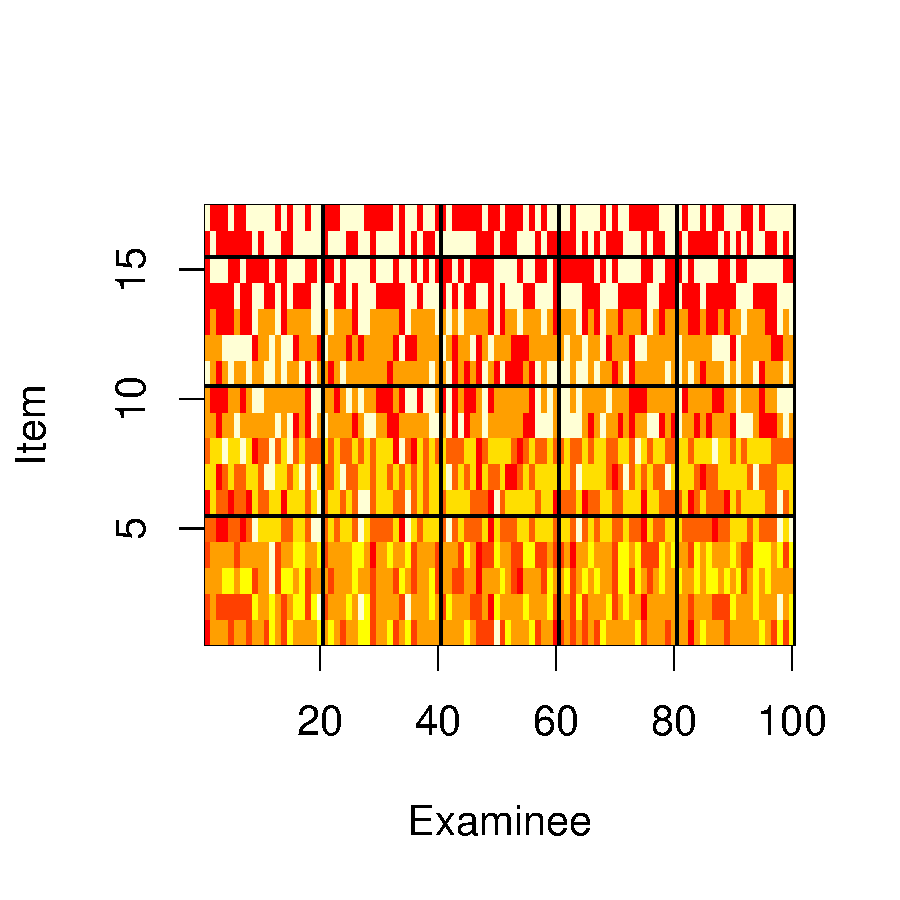
\includegraphics[scale =0.5] {NMFAddNonNoisy.pdf}\label{NMFAddNonNoisy}
 }\quad
&
\subfigure[Discretized result matrix with 20\% slip and 10\% guess factor]{
   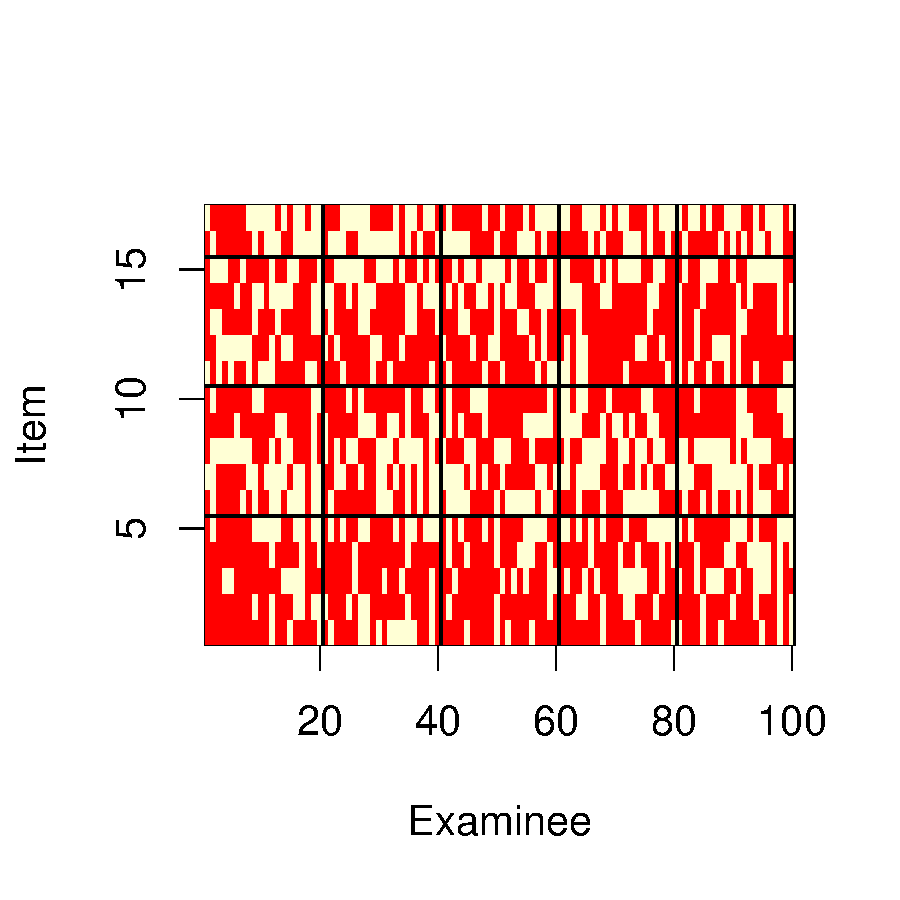
\includegraphics[scale =0.5] {NMFAddNoisy}\label{NMFAddNoisy}
 }\quad
\end{tabular}
\end{tabular}
\caption{Additive model of Q-matrix and Corresponding synthetic data}
\label{figNMFAddgen}
\end{figure}

Figure~\ref{figNMFAddQM} shows an additive type of Q-matrix and figure~\ref{NMFAddNoisy} is the result of cross product of this matrix to a students skills mastery matrix. Since the model is additive, there are some pale cells and the paler a cell is, the more chance a student has to success the question. In conjunctive model the result matrix is either $0$ or $1$. 

\section{DINA/DINO}

%mention that slip and guess are on items not students
These models are also categorized as linear models that use a Q-matrix. The Q-matrix can be predefined for a better comparison or can be synthetic. For synthetic Q-matrix we use the same method as described before. At the same time we can control the number of skills and items in generation of a Q-matrix.

Equation~\ref{DinoEQ3} requires three parameters to predict a test outcome. In our experiment we create a sequence of values for guess and slip in the range of $0$ and $0.2\%$. Examinee's skills can be generated by a normal distribution which should match the number of skills presented in the Q-matrix. The difference between creation of skills mastery matrix in DINA/DINO and NMF is the way that skills are appearing for each student. In DINA/DINO there is a predefined set of possible combination of skills that can be used in skills mastery for each student. For example for 3 skills, this set can have maximum 8 combination. There is a distribution that is assigned to this set which defines the probability of appearance for each combination in the skills mastery matrix. 
\begin{equation}
 P(X_{ij} \!=\! 1 \; | \; \xi_{ij}) \,=\, (1-s_j)^{\xi_{ij}} g_j^{1-\xi_{ij}}
\label{DinoEQ3}
\end{equation}
We can apply total success rate during the creation of student's skills mastery matrix where students skills define the success rate of a dataset. Since these models are behaving based on a single value that represents student ability, we need to calculate an array of abilities for each item given a set of skills for an student. In DINO we use a disjunction between skills of an item and skills of a student to determine whether the student has the ability or not where for DINA a conjunction applies.

\section{Educational data generator}

With all the parameters and models that were described, it is still challenging to generate synthetic data for a specific model with a set of given parameters. We \citep{Trieu2015} create a package that generates artificial data under a specific model's assumption given a set of parameters. Previous sections described the generation process for each model. This task is easy and possible as long as two conditions are satisfied : 
\begin{itemize}
\item First: All the parameters for a model are given. Table \ref{tbl:param-DataGen} shows a list of required parameters to generate artificial data.
\item Second: There exists no conflict between the given parameters. For example given ``number of skills'' as a parameter equal to $4$ and a predefined ``Q-matrix'' with $5$ skills is a conflict to generate a synthetic data based on DINO model. However, testing these conflicts is not an easy task and also resolving a conflict is another challenge.
\end{itemize} 

There exists a hierarchical structure among parameters of a model. Some lower level parameters can generate more complex ones which are included in the set of parameters that directly generates data. This process requires default values and distributions. Namely, given the number of items, skills and students, the Q-matrix and skills mastery matrix can be generated with a default normal distribution on items difficulty and students ability. Hence,  generating a dataset based on NMF conjunctive model will be possible since the prerequisite parameters are available. Therefore there are different combination of the sufficient parameters to generate a data based on a model. For example for a synthetic data with DINO model this set can be {Q-matrix, Skills mastery matrix, Slip and Guess vectors} or {Number of skills, Items and students}.

Given the tow conditions are satisfied, there would be different ways to generate data depending on the available set of parameters
%One can conclude from the above observation that there are many different ways to generate data depending on which model is being acquired and which parameters are given (assuming that they all satisfy condition 1 and condition 2). At this point it is important to stress that for different sufficient and consistent sets of parameters, even with respect to a single model M, we must expect different amounts of variance in the generated data. The reason is, with a set of parameters at lower level, it requires more intermediate generating steps before reaching the final one (generating data), thus produces more variability in the corresponding generated data.

%R package edmsyn provides users a simple framework that conveniently handles all the situations above while generating data, including checking for condition 1 and condition 2. It also automates the process of learning parameters from raw data, modifying and using this information to create synthetic data from 10 different models. This document is intended to give a quick and thorough tutorial on using edmsyn.


%Since some of the parameters are shared between different models, edmsyn did not regard the collection of all parameters from 10 models separately, but jointly as different aspects describing a single instance of reality. For example, the vector of discrimination factors of all items is a parameter belongs to the IRT-2pl model, which is not the case for the parameter Q-matrix, however, edmsyn introduces the class context where these two parameters co-exist in a single object and can be utilized according to user purpose.

